	This Section explores Blaise and SurveyMonkey architectures in order to determine the architectural properties being adopted by \gls{cawi} systems. However, other software solutions such as \gls{cases}, have not been explored due to the absence of publicly available documentation.

	\subsubsection{Blaise}\label{sec:literature:blaise}
	%This style permits developers to focus on a specific role, i.e. they can implement and maintain isolated services, multiple applications can reuse services code and the testability is improved.
	The architecture style of Blaise is \gls{wcf}, which is an implementation of \gls{soa}. In this style, the interactions among components is carried out by sending data through asynchronous messages that can be either \gls{xml} formatted or using complex streams of binary data. The \gls{cawi} solution offered by Blaise, separates the functionalities into different roles (see Figure \ref{fig:literature:soaBlaise}) \cite{proc:segel15}. The most important server roles are: \emph{survey manager}, that holds the creation and publishing of surveys; \emph{data entry server}, used to validate input and routing logic; \emph{data server}, that performs read/write operations into the databases; \emph{session server}, that stores and controls the active interviews; and \emph{web server} used to host and serve web pages to the end users. %This role uses the \gls{mvc} design pattern that offers benefits such as loose coupling due to the separation of concerns, it helps to manage the application when becomes more complex or promotes parallel development (e.g. one developer can focus on the model, a second can concentrate on the controller and a third one on the view). Nevertheless, we consider that this component can be moved to the client-side since browsers nowadays have mature JavaScript frameworks able to apply this design pattern. Hence, this suggestion may produce a much better user experience and help to reduce network latency since only data in \gls{json} or \gls{xml} format is sent.

	\begin{figure}[h]
	\centering
	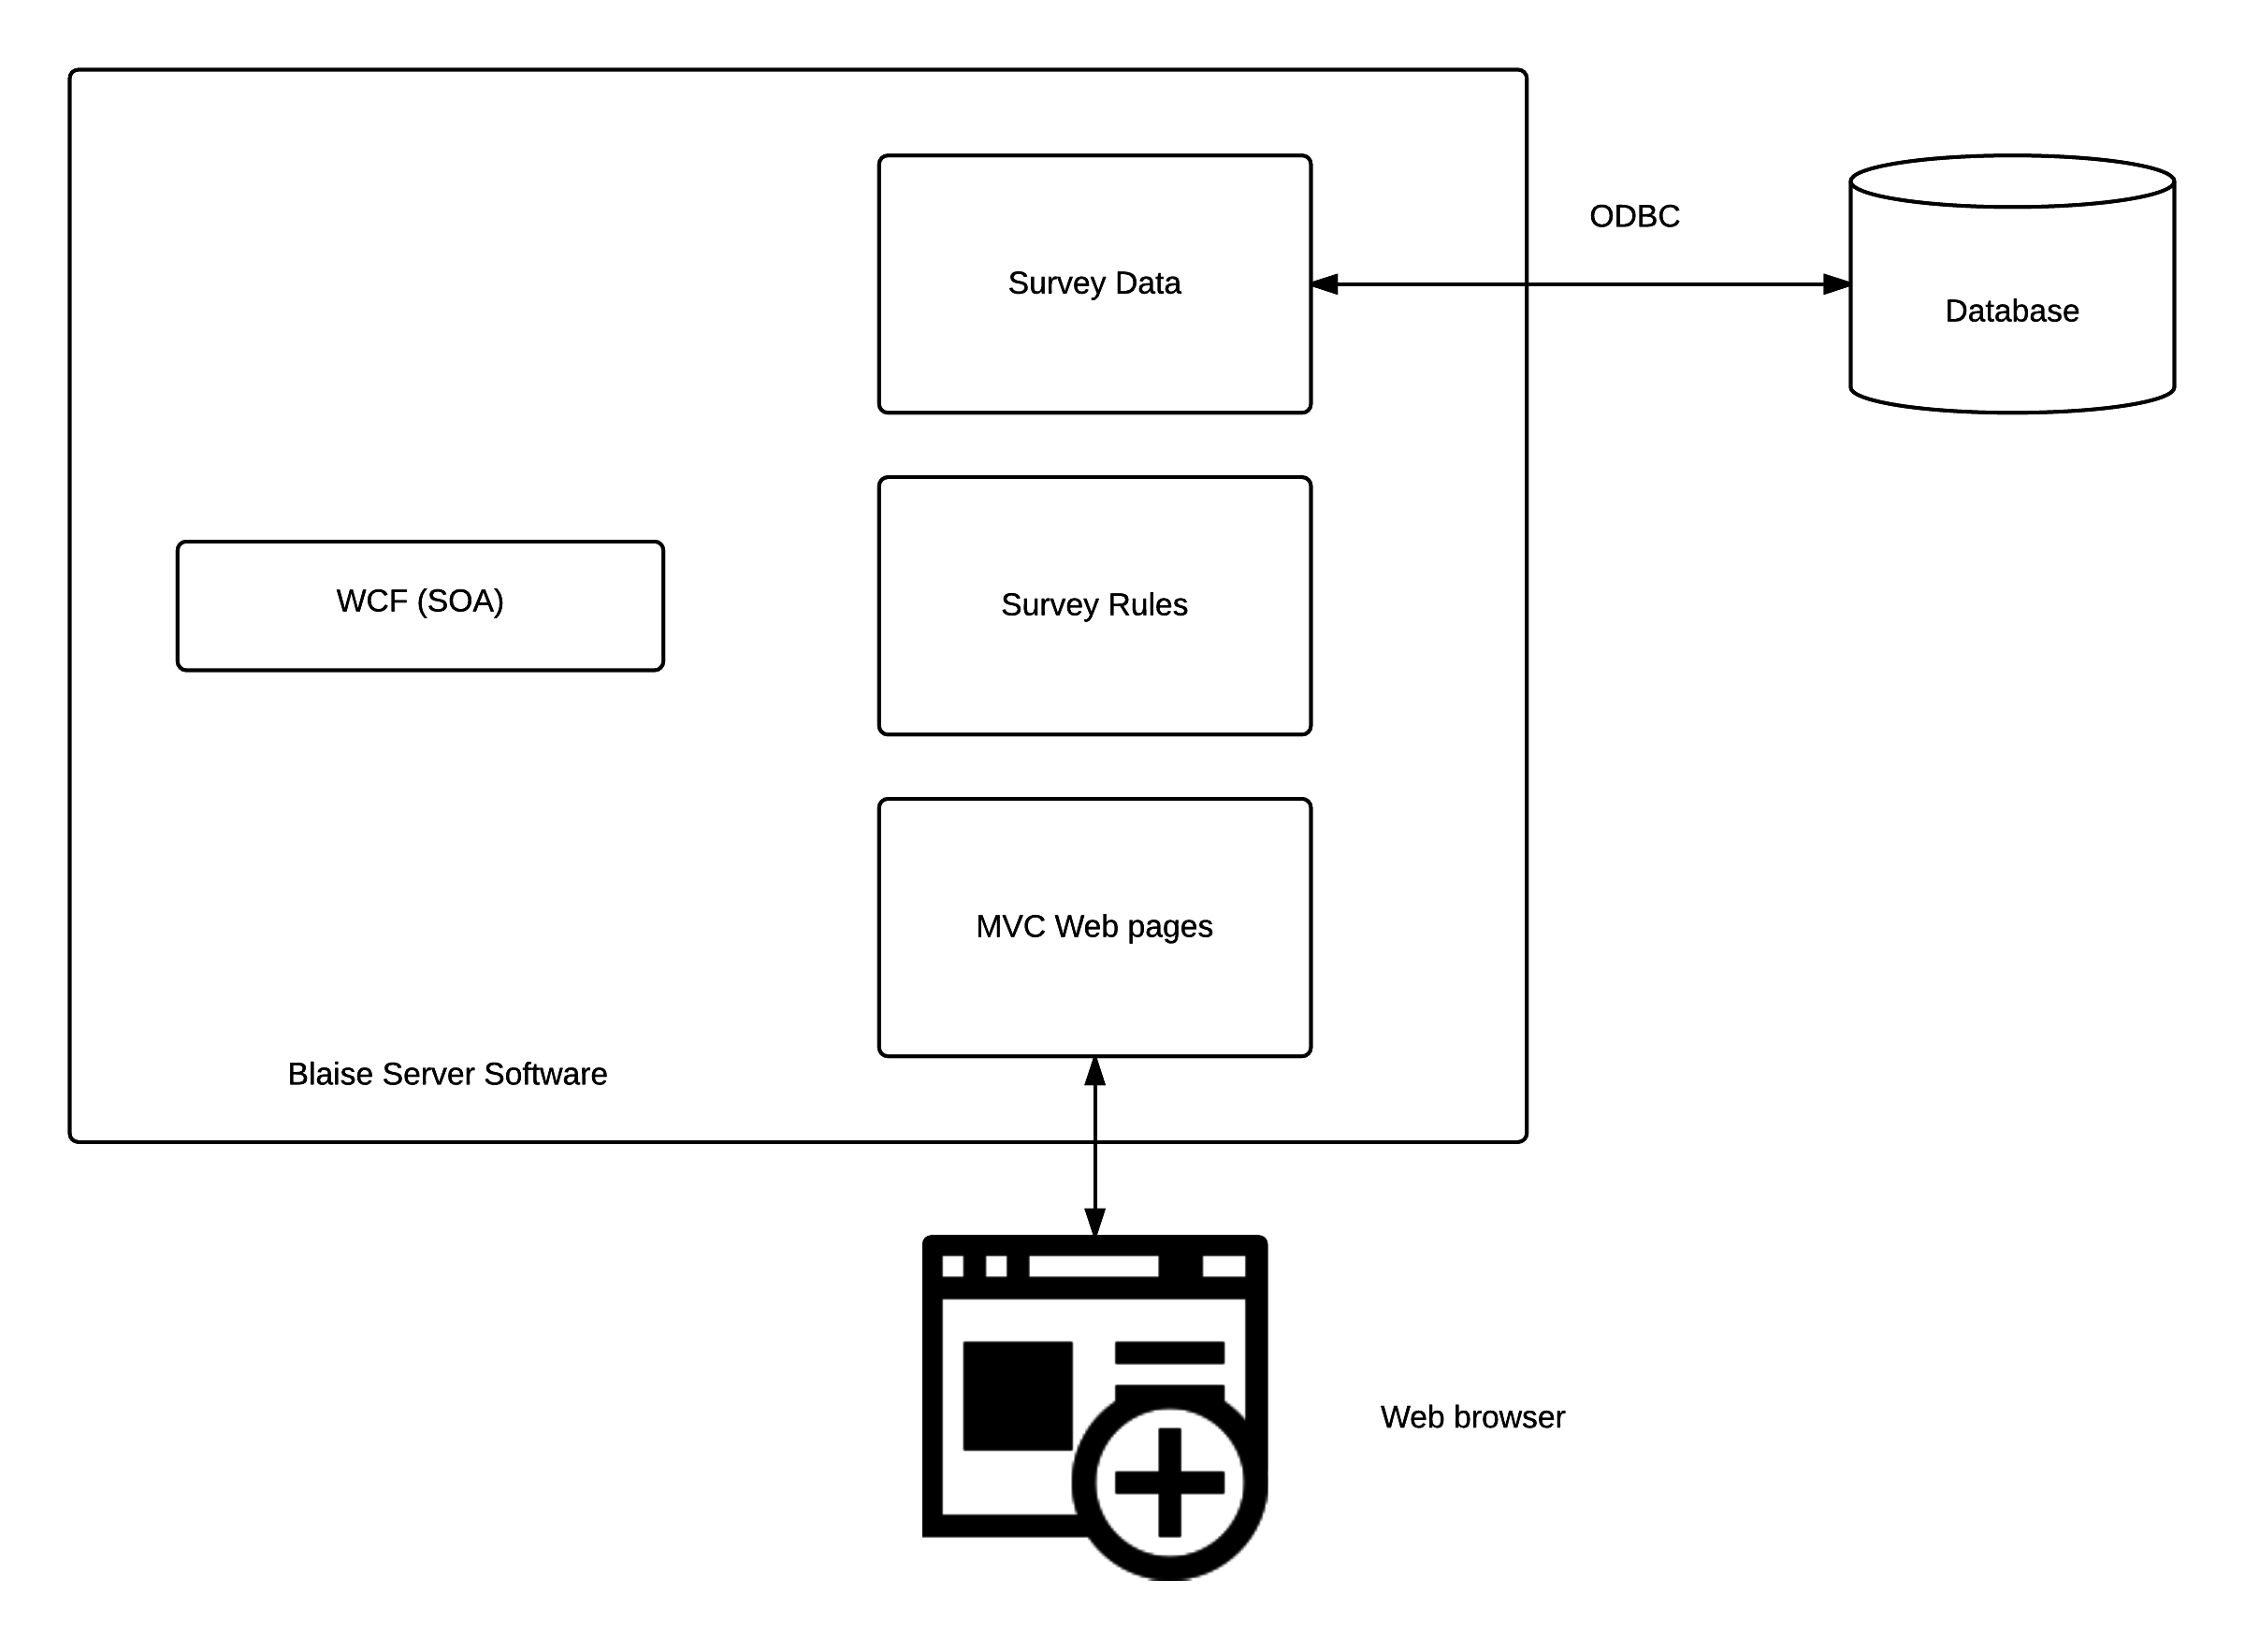
\includegraphics[max size={\textwidth}{\textheight}]{literature/img/soaBlaise.png}
	\caption{Blaise Architecture}
	\label{fig:literature:soaBlaise}
	\end{figure}

	The \gls{wcf} architecture style of Blaise induces simplicity by making a clear separation of concerns that leads to have services less complex and interdependent. Additionally, as this approach defines interfaces to communicate the different roles, any change at any component should not impact negatively into its consumers. However, the portability, reliability and scalability are not carefully considered. Specifically, the portability is not present due to the platform-dependent architecture of \gls{wcf} that only works under Microsoft environments. Regarding the reliability, it may be affected by the fact that the data server role makes the entire system vulnerable under any failure due to its inability to be set up with multiple physical or virtual machines \cite{proc:volguine13}. In respect to the scalability, the presence of a session server role to keep the state of every interview ongoing, not only prevents the server to free resources but also makes it harder to manage, replicate and synchronise state changes under a multi-server configuration.

	\subsubsection{SurveyMonkey}\label{sec:literature:surveyMonkey}
	%http://www.slideshare.net/mingli.yuan/a-brief-introduce-to-wsgi
	%http://agiliq.com/blog/2013/07/basics-wsgi/
	%https://developer.surveymonkey.com/api/v3/#authentication
	SurveyMonkey is the world's largest survey company \cite{web:groom14}. Its \gls{cawi} solution is written in Python and its core features are separated into different services. Most of the services communicate through a \gls{json} web \gls{api} over \gls{http}/\gls{http}S. SurveyMonkey implements \gls{soa} through \gls{wsgi} (see Figure \ref{fig:literature:surveyMonkey}). In this style, the web server is set up to receive client's requests and return responses back. The web server itself, does not directly creates a response but invokes the web application that produces a response based on the \gls{url} requested and pass it back to the web server. The server ultimately sends to the client. The \gls{wsgi} specifies the rules that need to be implemented by both sides, i.e. the web server and \gls{mvc} Framework. SurveyMonkey utilises Pyramid as the web application framework to produce many of its services.

	\begin{figure}[h]
	\centering
	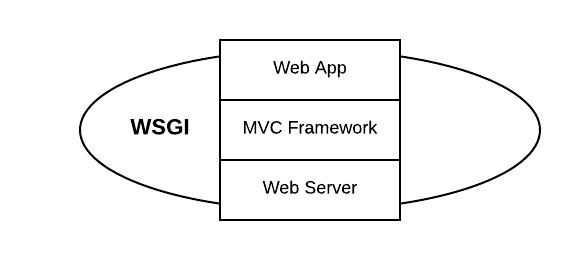
\includegraphics[width=0.75\textwidth]{literature/img/surveyMonkey.png}
	\caption{SurveyMonkey Architecture}
	\label{fig:literature:surveyMonkey}
	\end{figure}

	The \gls{wsgi} architecture style of SurveyMonkey induces simplicity and scalability. The simplicity is achieved through the use of pyramid \gls{mvc} web framework which permits loose coupling due to the separation of concerns. This software pattern, promotes parallel development (e.g. developers may focus on models, controllers or views). Regarding the scalability, unlike Blaise, there is no session persisted on the server, i.e. its stateless configuration based on a token-based authentication, promotes flexibility to scale. In respect to the portability, the application code is written in a cross-platform language, however we have not found enough information to determine whether or not the reliability or portability are induced. %For instance, the lack of awareness regarding its database solution


